% Chapter Template

\chapter{Literature Review} % Main chapter title
%this should end up being roughly 10 pages


\label{Chapter2} % Change X to a consecutive number; for referencing this chapter elsewhere, use \ref{ChapterX}

%----------------------------------------------------------------------------------------
%	SECTION 1
%----------------------------------------------------------------------------------------
\section{Measurement and Modeling of Riots and Protests}

Riots and protests constitute integral components of democratic societies \citep{anderson2006learning}, yet it is imperative for government authorities to effectively mitigate the economic and human costs that may be associated with these events to maintain stable governance \citep{klein2018dynamics}.  This is accentuated by the heightened prevalence of protests and riots on a global scale in recent years \citep{ciorciari2016nationalist}.  One viable strategy for authorities to temper the negative impacts of these events is through preemptive allocation of resources, such as medical units \citep{gong2007allocation} or increased international presence (i.e., U.N. peacekeepers) in anticipation of unrest \citep{greer2010we}.  At the international scale, in an attempt to protect citizens who are traveling abroad, responsible governmental foreign offices (the US Department of State as an example) may also issue travel warnings for particular areas to avoid \citep{lowenheim2007responsibility}.  However, proactive approaches necessitate the capacity to predict both the time and location of potential conflict events \citep{wu2017forecasting}.

A number of approaches exist which aid in the measurement and prediction of protests or riots \citep{wu2017forecasting}.  Past literature, for instance, has demonstrated the utility of news reports in providing valuable insights into civil conflict, such as riots and protests in response to rising food prices \citep{heslin2021riots}.  Using this approach, studying riots in France, researchers were able to replicate the spread of riots using an epidemic-like model with as few as six parameters that included population demographics, police reports, and spatial information \citep{bonnasse2018epidemiological}.  Social media platforms represent another venue for authorities to detect and analyze real-world events, including social unrest like riots and protests \citep{becker2011beyond, korolov2016predicting, petrovic2010streaming}.  X (formerly Twitter) is a common focus of these studies, and can be used as a near real-time reporting source \citep{becker2011beyond}.  Analysis of twitter data has demonstrated the correlative relationship between daily hashtag use and protests, predicting protests 24-48 hours prior to occurring in Baltimore and New York City during 2015 \citep{korolov2016predicting}.  Prior work in this field has show the ability to predict the probability of fatalities associated with conflict events using satellite imagery, within conflict areas in Nigeria, with accuracy rates of 80\% when combining Landsat imagery and CNNs \citep{goodman2021convolutional}. 

Much of the current research in forecasting social unrest is focused on the likelihood of a future event \citep{renaud2019social, phillips2017using, cadena2015forecasting, filchenkov2014more, compton2013detecting}.  There are other efforts to better understand and model the characteristics of smaller sub-events within broader riots, such as shooting or fires \citep{alsaedi2017can}.  Modeling of riots demonstrates an ability to accurately simulate many of the spatial characteristics of riots, including the distance participants will travel within contiguous riot areas \citep{davies2013mathematical}.  Beyond riot forecasting, tweet analysis demonstrates the ability to detect and discriminate between disruptive events within a riot and normal information dissemination \citep{alsaedi2015identifying}.  Additionally, when analyzing individual behavior, social media has been studied to demonstrate not only how information is distributed about future and concurrent protests, but also how individuals are recruited into protesting \citep{gonzalez2011dynamics}.

The accuracy and spatial specificity of existing riot and protest forecasting techniques vary.  Previous research has shown that leveraging information from social media (i.e., Tweets) can result in the accurate prediction of riots in some cities (i.e., Baltimore and New York City), but these models require location-specific information or hashtags which inhibit their use in other settings (i.e., San Francisco) \citep{korolov2016predicting}.  Related tweet-based analyses have shown that accurate temporal estimates across broad geographies are possible, but without spatial specificity in where riots or protests are likely to occur \citep{gonzalez2011dynamics}. Other researchers have used a broader range of sources to achieve higher spatio-temporal accuracy, such as police reports, but these techniques are inherently limited to a small number of areas where such information is available \citep{alsaedi2015identifying,korolov2016predicting,gonzalez2011dynamics,bonnasse2018epidemiological, alsaedi2017can}.

\section{Satellite Imagery}

There is a long history of utilizing satellite imagery in research that is based on visually observable characteristics, such as habitat and land cover change \citep{alo2008identifying,stow2008monitoring,rogan2004remote}, soil evaluation \citep{foody2004toward}, and urban land cover \citep{zhou2008object}.  When satellite imagery is used in conjunction with deep learning techniques, including CNNs, researchers have recently been able to learn about topics not normally associated with traditional satellite imagery uses, such as predicting crime \citep{najjar2018crime} or the prevalence of cancer \citep{bibault2020deep}.  Other examples include estimating human migratory flows \citep{runfola2022deep}, estimating educational outcomes \citep{runfola2022using}, tracking economic growth in China \citep{brewer2023tracking}, predicting road quality \citep{brewer2021predicting}, and estimating socioeconomic census variables from satellite imagery \citep{runfola2024multi}.

The ability to estimate income with satellite imagery is one of the most commonly studied topics, with researchers initially exploring the use of nighttime lights as a proxy for development \citep{elvidge2012night}.  Building on these approaches, researchers leveraged a CNN in conjunction with both daytime satellite imagery and nighttime lights, an approach which was able to explain up to 75\% of the of the variation of household wealth in various countries that lacked detailed survey data \citep{jean2016combining}.  A similar CNN-based approach was able to leverage satellite imagery to predict GDP and total retail sales with a Pearson coefficient of 0.85 for both tasks, outperforming linear regression models \citep{wu2019estimation}. CNNs that were trained on higher resolution imagery were able to explain 57\% of the variation in poverty of municipalities in Mexico \citep{babenko2017poverty}.  These authors used two different satellite image sources, MAXAR (formerly Digital Globe) and Planet, noting a slight decrease in performance of Planet imagery but highlighting the benefit of Planet's daily image capability.  When using publicly available satellite imagery with CNNs, researchers were also able to predict school test scores with accuracy's between 76\% to 80\% with images of the schools \citep{runfola2022using}.  Even human migratory flows have been predicted with an accuracy of $\ R^{2}= 0.72$ when satellite imagery and and census data are used in conjunction with CNNs, which outperforms the use of socioeconomic census data alone \citep{runfola2022deep}.  Some of the most recent literature on this topic has explored the ability of CNN based satellite models to estimate broader ranges of census variables in regions that may lack regular census instruments \citep{runfola2024multi}.

In scenarios where data is challenging or impossible (i.e., historic time periods) to collect, there is increasing evidence that satellite imagery can aid in filling data gaps \citep{goodman2021convolutional,jean2016combining,bharti2018fluctuations,hu2019mapping, aung2021using}.  This characteristics of satellite information is important in the context of studying riots and protests, as the majority of literature we've identified has focused on the use of news or social media sources \citep{purbrick2019report, greer2010we, wu2017forecasting, ciorciari2016nationalist, becker2011beyond, korolov2016predicting, renaud2019social, phillips2017using, cadena2015forecasting, filchenkov2014more, compton2013detecting, alsaedi2017can}.  There are many countries of research interest that do not allow free access to social media or control the news narrative, such as Russia \citep{gehlbach2010reflections}, China \citep{tai2014china}, Iran \citep{rahimi2015censorship}, and Venezuela \citep{pain2021everything}.  Satellite imagery provides a unique capability to access data in a country that might restrict access to social media or control news sources, motivating us to use satellite imagery to predict conflict. 

There a many options to consider when using satellite imagery, \citep{kramer2008overview}.  A comprehensive evaluation of which imagery product to use broadly includes a consideration of it's spatial and spectral resolution, temporal revisit times, and radiometric precision \citep{xie2008remote}.  A number of satellites and sensors have been launched over the last four decades, with many of these still providing regular imagery today.  A list of potential sources for imagery is shown in table \ref{tab:sat_options} 


\begin{table}
\centering
\begin{tabular}{ |l||l|l|l|  }

\hline
 \textbf{Source} & \textbf{Number of Bands} & \textbf{Resolution} & \textbf{Revisit Time} \\
 \hline
 Landsat 9 & 9 spectral bands  & 30m & 16 Days \\
 \hline
  Sentinel-2 & 4 bands & 10m & 5 Days \\
 \hline
  SPOT-6 &  4 bands & 6m & 26 days \\
 \hline
 PlanetScope & 8 spectral bands & 3-4m & Daily \\
 \hline
 GeoEye-1 & 4 bands & 1.84m  & 2-3 Days \\
 \hline
 WorldView-3 & 8 spectral bands & 0.31m & 1-4 Days\\
 \hline


\end{tabular}
\caption{Landsat data is for Landsat 9 \citep{USGSlandsat}; Planet data is for PlanetScope \citep{planetScope}; WorldView-3 data can be found at \citep{maxar_worldview3}; GeoEye-1 data can be found at \citep{maxar_geoeye}; Sentinel-2 data can be found at \citep{copernicus_sentinel2}; SPOT-5 data can be found at \citep{spot6_esa} }
\label{tab:sat_options}
\end{table}

In this dissertation, we focus on the use of PlanetScope, a product provided by the commercial provider \textit{Planet}. PlanetScope is a constellation of approximately 130 satellites, cumulatively capable of taking approximately 3-4 meter pixel resolution images across the landmass of the Earth each day \citep{planet}.  To date there have been three generations of PlanetScope satellites, that have images dating back to July 2014.  All three generations of the satellites have produced 3 band imagery (red, green, blue, channels), with the newest generation collecting 8 bands \citep{planet}.  Each image covers between 25 x 11.5 km to 32.5 x 19.6 km, depending on the sensor used (\cite{planet}; see table \ref{tab:planetscope_ch2} for more details).  In order to leverage the full length of time covered in our record of conflict events (see Chapter 3), we will use only the Red, Green, and Blue bands of data that have been provided by the earliest Dove Classic, Dove-R, and newest SuperDove satellites.  An example of an image from Planet is shown in figure \ref{fig:athens_baseimage_ch2}.


\begin{figure}
    \centering
    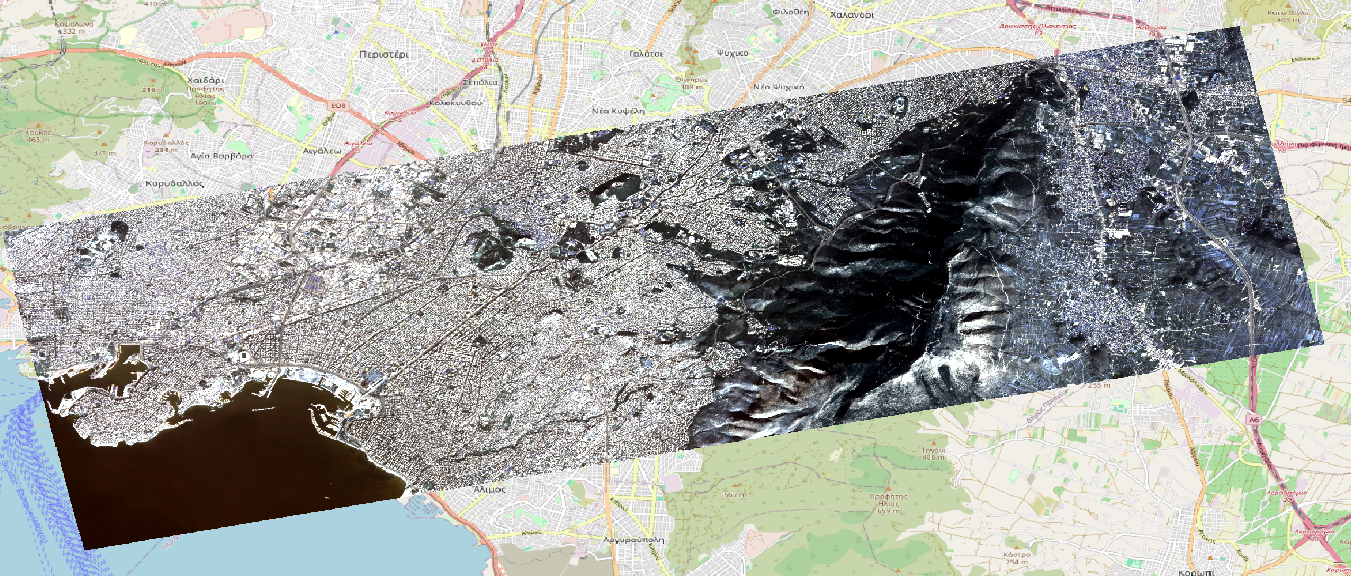
\includegraphics[width=1\linewidth]{athens_greece_satimage.png}
    \caption{Satellite Image of Athens Greece, taken 31 January 2018. Imagery \textcopyright Planet Labs PBC 2023. All rights reserved.}
    \label{fig:athens_baseimage_ch2}
\end{figure}

\begin{table}
    \centering
    \begin{tabular}{|l|c|c|c|}
        \hline
            & \textbf{Dove Classic} & \textbf{Dove-R} & \textbf{SuperDove}\\
            \hline
         Band  & Wavelength (nm) & Wavelength (nm) & Wavelength (nm) \\
         \hline
         Red   & 590 - 670       & 650 - 682       & 650 - 680\\
         Green & 500 - 590       & 547 - 585       & 547 - 583\\
         Blue  & 455 - 515       & 464 - 517       & 465 - 515\\
         \hline\hline
         Image Area &  25 x 11.5 sq km & 25 x 23 sq km &32.5 x 19.6 sq km\\ \hline
         Availability & July 2014 - April 2022 & March 2019 - April 2022 & March 2020 - present \\ \hline
         
    \end{tabular}
    \caption{Technical Data from Planet about Planetscope\citep{planetScope}. As the Planetscope satellites have increased their capabilities over time, the technical specifications have slightly shifted.  Later generations of the satellites have more bands available, but to maintain continuity over our data set, we are only considering RGB bands. }
    \label{tab:planetscope_ch2}
\end{table}

\section{Convolutional Modeling}
Computer vision is a branch of machine learning that attempts to train computers to visually learn and identify objects similar to vision in humans \citep{goodfellow2016deep}.  Early attempts in this field were pioneered by Rosenblatt using perceptrons to attempt to identify letters visually \citep{rosenblatt1957perceptron}.  These early concepts, like perceptron, would develop and advance towards modern applications and the various forms of Deep Neural Networks \citep{fradkov2020early}.  These neural networks were not limited to a single perceptron or neuron, but could have many layers with complex connections among the layers.  Computational power and speed has improved significantly since the 1950s \citep{nordhaus2001progress}, and so has the advancement of neural networks.  

In this study, we rely on convolutional neural networks (CNN), a type of deep learning that is designed for the analysis of image data. These techniques have been shown to be effective at detecting, labeling and differentiating objects \citep{simonyan2014very, zhang2016deep, he2016deep, krizhevsky2017imagenet, voulodimos2018deep}.  CNNs represent a family of deep learning techniques that implement convolutional layers that extract features from an image \citep{zhang2016deep}.  There are many types of CNN architectures that have performed well across a wide range of computer vision tasks \citep{voulodimos2018deep,simonyan2014very,szegedy2015going}.  In general, convolutional networks refer to functions that take image inputs and kernels to generate outputs known as feature maps \citep{goodfellow2016deep}.  A formal definition is shown in formula \ref{cnn_def}.  The feature map, $\ S(i,j)$, is the output of image \textit{I} with dimensions \textit{i,j}, convolved with kernel \textit{K} with dimensions \textit{m,n} \citep{goodfellow2016deep}.  

\begin{equation}
S(i,j) = (K * I)(i,j) = \sum_{m} \sum_{n} I(i-m,j-n)K(m,n) 
%\caption{Formal definition of a convolution.  The feature map , $\ S(i,j)$, is the output of image \textit{I} with dimensions \textit{i,j}, convolved with kernel \textit{K} with dimensions \textit{m,n} \citep{goodfellow2016deep}.  }
\label{cnn_def}
\end{equation}

An early CNN  that leveraged GPUs was AlexNet \citep{krizhevsky2017imagenet}.  The architecture of AlexNet comprises five convolutional layers and three fully connected layers. Despite its relatively shallow structure, this network exhibits exceptional performance and played a crucial role in promoting the adoption of CNNs in computer vision. Notably, advancements in AlexNet demonstrated that the integration of dense convolutional layers could enhance performance \citep{szegedy2015going}.  A diagram of the architecture of AlexNet is displayed in figure \ref{fig:alexnet_architecture}.  

\begin{figure}
    \centering
    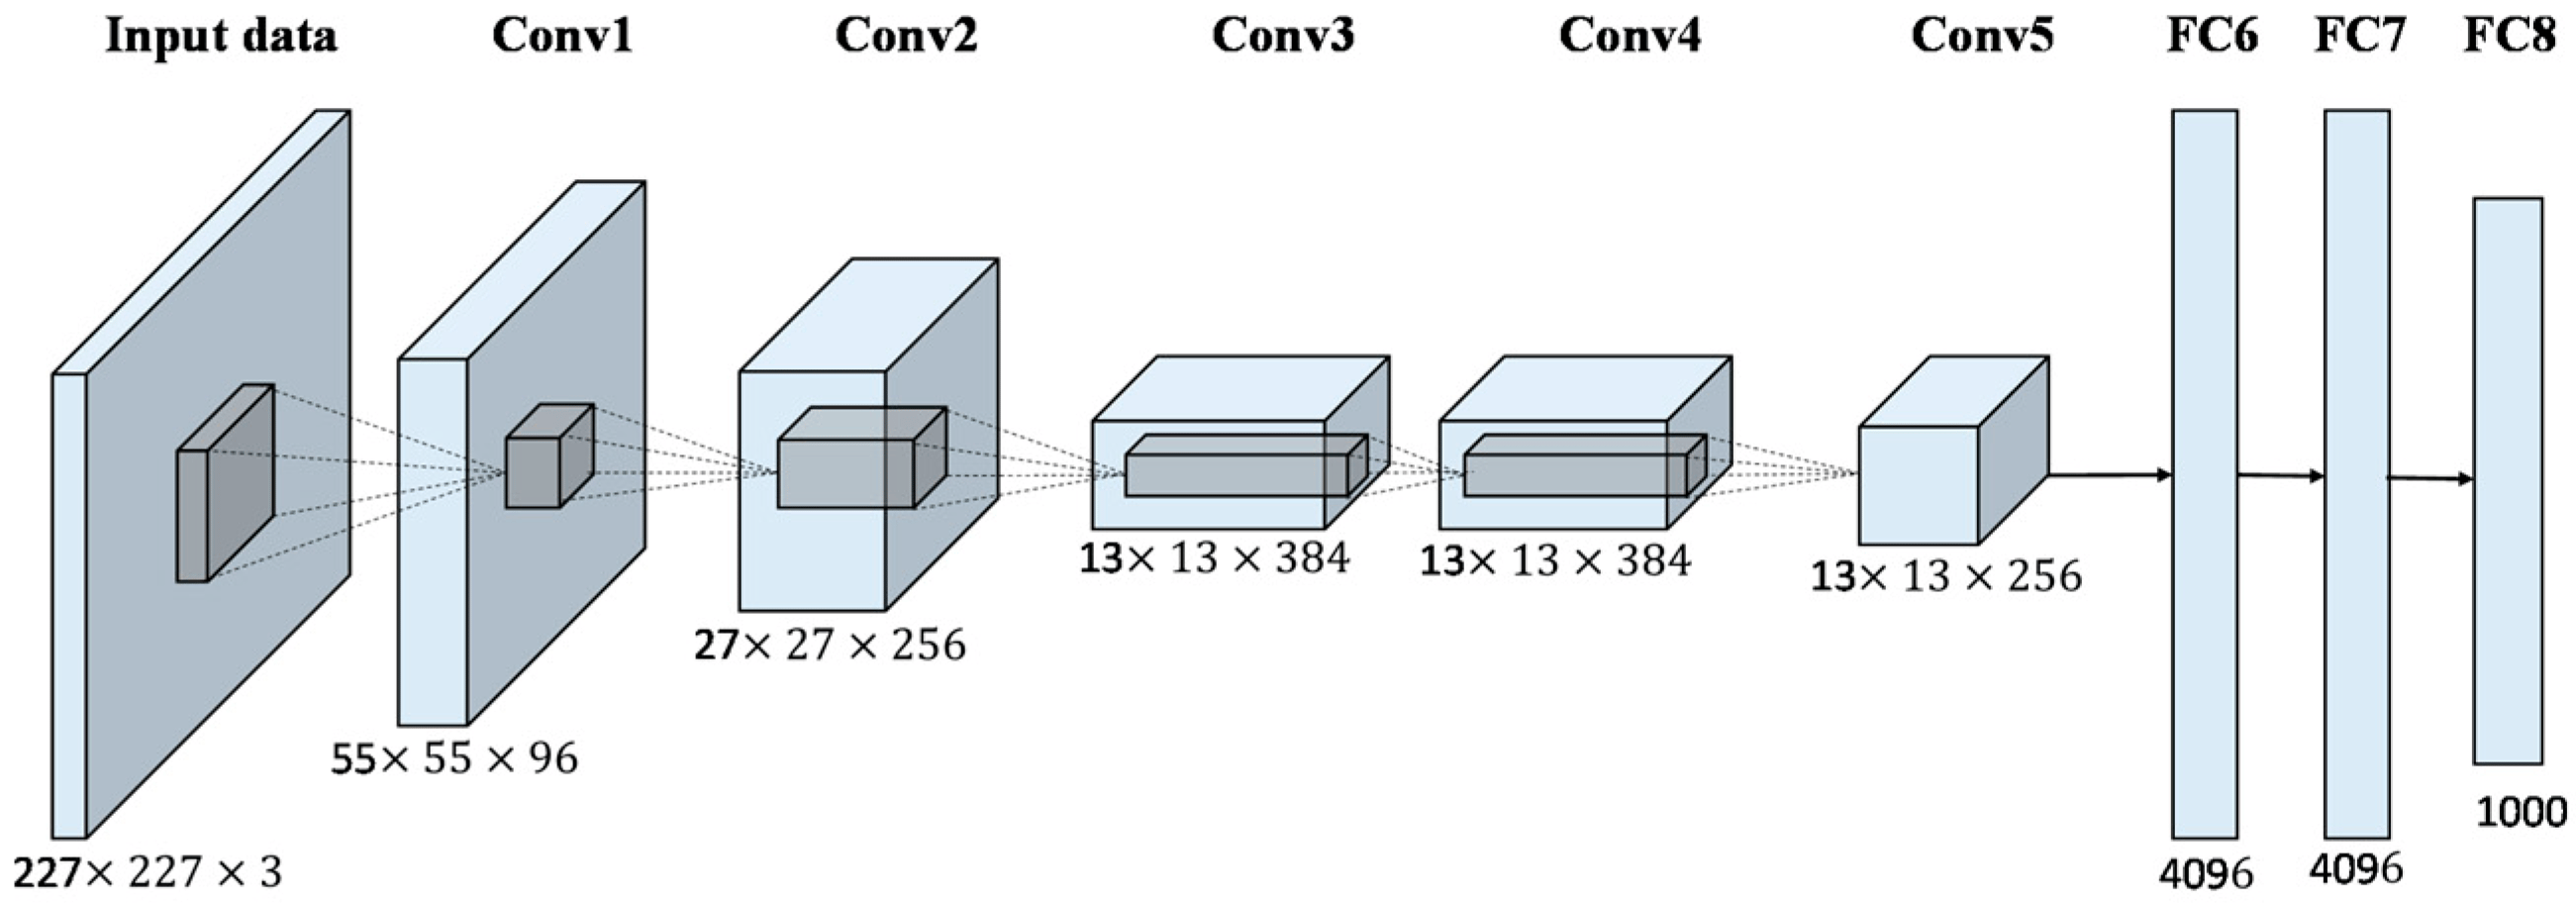
\includegraphics[width=0.5\linewidth]{Figures/alexnet_architecture.png}
    \caption{Architecture of AlexNet, highlighting input data passing through five convolutional layers and 3 fully connected layers.  Figure is from \citep{han2017pre}.}
    \label{fig:alexnet_architecture}
\end{figure}

Building upon this progress, a novel CNN named VGG was introduced by the vision geometry group at the University of Oxford \citep{simonyan2014very}. The VGG architecture emphasizes stacked convolutional layers with smaller kernel sizes, departing from individual convolutional layers with larger kernels. This approach yields significant computational gains and enables a more discriminative decision function through heightened non-linearity. Subsequent modifications and refinements to the VGG implementation have further improved the architecture's performance \citep{hu2018squeeze}.  A diagram of VGG is shown in figure \ref{fig:vgg_architecture}.

\begin{figure}
    \centering
    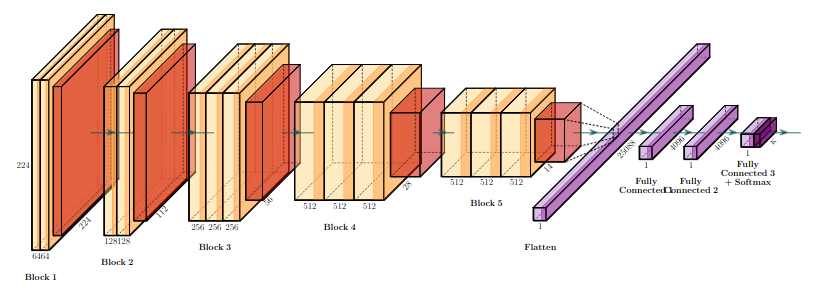
\includegraphics[width=0.5\linewidth]{Figures/vgg_architecture.png}
    \caption{Architecture of VGG, highlighting input data passing through stacked convolutional layers before flattening and passing through fully connected layers.  Figure is from \citep{vrbancic2019transfer}.}
    \label{fig:vgg_architecture}
\end{figure}

As VGG was developed, a desire to test so-called `deeper' networks took hold as a potential route forward for improved levels of capability \citep{simonyan2014very}.  However, VGG, AlexNet, and other earlier networks were functionally limited in the depth they could achieve due to - at the time - the difficulty of optimizing deep networks due to vanishing gradients \citep{he2016deep}.  ResNet, short for residual convolutional neural network, was developed to address the challenges associated with deeper networks while aiming to improve accuracy. A notable characteristic of ResNets is the inclusion of residual connections, which establish a direct path from one layer to deeper layers, bypassing intermediate convolutions (see figure \ref{fig:residual_block}). By incorporating these residual connections, the network can increase in depth without encountering issues related to gradient back propagation during optimization \citep{he2016deep}. Following the initial introduction of ResNets by He et al., subsequent researchers have made various improvements and modifications, often altering specific dimensions while preserving the general ResNet structure \citep{xie2017aggregated,zagoruyko2016wide}. Furthermore, others have explored alternative approaches to enhance the training process or optimize the loss functions employed in ResNets \citep{he2016identity,huang2016deep,he2019bag,wightman2021resnet}. The concept of forwarding information through skip connections has also been expanded into fully connected dense blocks in the DenseNet architecture \citep{huang2017densely}. Due to their remarkable effectiveness, ResNets have emerged as one of the dominant CNN architectures widely employed in contemporary deep learning applications.

\begin{figure}
    \centering
    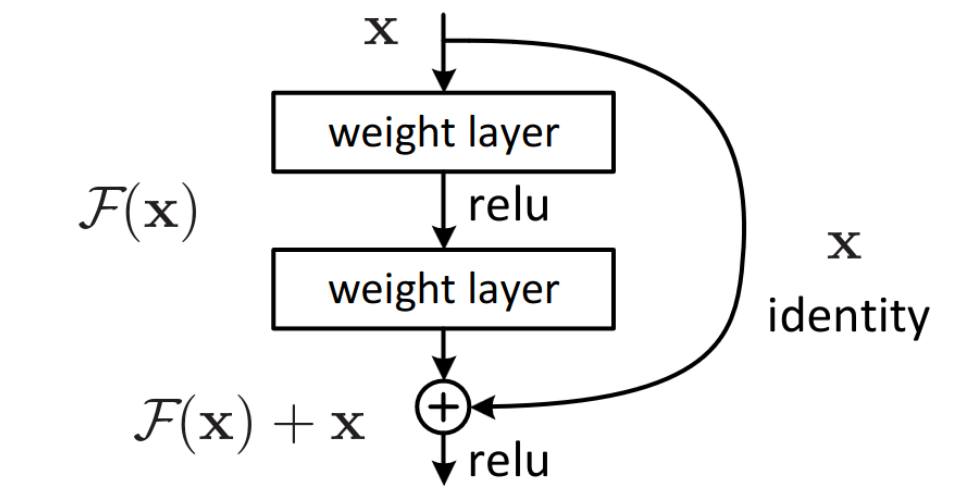
\includegraphics[width=0.5\linewidth]{Figures/residual_learning_block.png}
    \caption{Residual learning block, highlighting information flow deeper into networks that by passes itermediate layers.  Figure is from \citep{he2016deep}.}
    \label{fig:residual_block}
\end{figure}


\begin{figure}
    \centering
    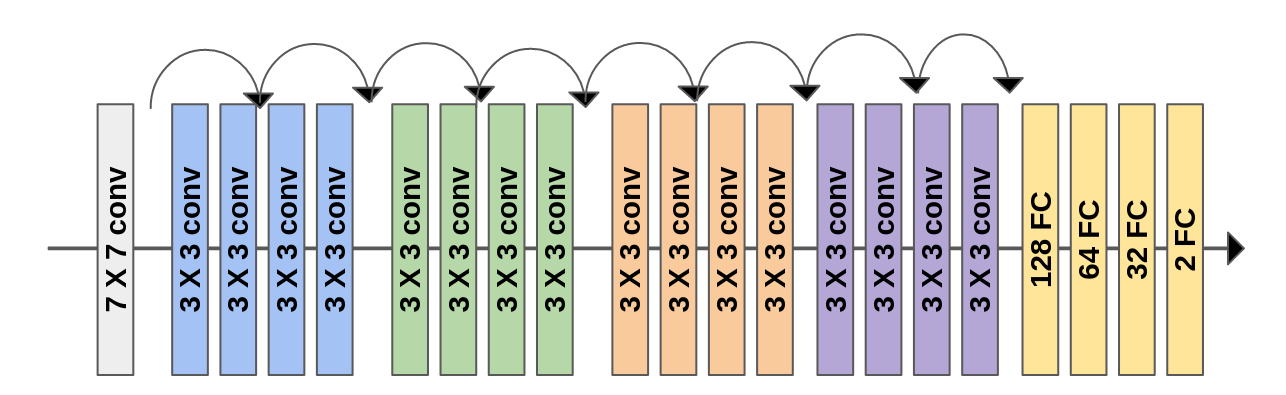
\includegraphics[width=1\linewidth]{Figures/resnet18_architecture.png}
    \caption{ResNet18, highlighting stacked convolutional layers, with residual learning depicted between intermediate convolutional layers.}
    \label{fig:resnet18_ch2}
\end{figure}

By 2016, ResNet architectures reached depths of 1001 layers, and achieved error percentages as low as 4.62\% on CIFAR-10 and 22.71\% on CIFAR-100 \citep{xie2017aggregated}.  Research has demonstrated ResNet-18's ability to identify cancer from x-ray images with 84\% accuracy \citep{khan2018evaluating}.  Various ResNet architectures have demonstrated the ability to semantically segment satellite imagery with accuracy over 80\%, depending on the specific architecture \citep{heryadi2020effect}.  While it is accepted that deeper neural networks tend to perform better under some circumstances \citep{he2016deep, lodhi2019multipath, sinha2020d2rl}, there can be benefits to using a shallower networks in some scenarios \citep{sekiyama2018profile,gorban2020deep}. 


\section{Explainability}

It is not uncommon for deep neural networks to be refereed to as "black boxes" \citep{dabkowski2017real,fong2017interpretable,petsiuk2018rise,chattopadhay2018grad,naidu2020cam}, due to the challenge of understanding why a model performs the way it does.  This is a particularly notable challenge in the field of computer vision, where an algorithm may leverage unexpected features to distinguish between cases \citep{wei2018deep}. 
\par
There have been multiple attempts to provide semantically-interpretable descriptions of what features are most important within a target image; these include analyzing intermediate convolutional layers \citep{zeiler2014visualizing}, inverting convolutional networks to understand image salience \citep{mahendran2015understanding,dosovitskiy2016inverting}, and Class Activation Mapping (CAM) \citep{zhou2016learning}.  Grad-CAM, introduced in \citep{selvaraju2017grad}, was able to generalize CAM for use in more deep learning models, by analyzing the gradients in the last convolutional layer to create a visualization indicating what regions in the original image are important for classification.  An example of Grad-CAM is displayed in figure \ref{fig:gradcam_introduced}.

\begin{figure}
    \centering
    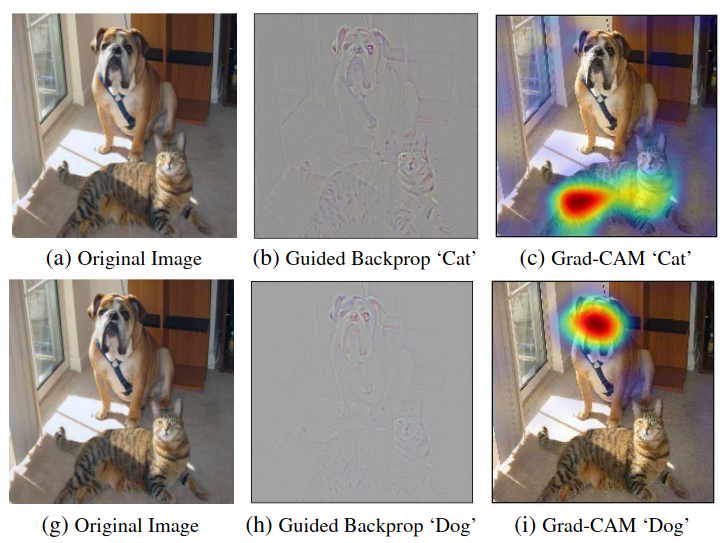
\includegraphics[width=0.5\linewidth]{Figures/gradcam_example.png}
    \caption{Images displaying the results of Grad-CAM analysis.  This example shows the ability of CAM techniques to highlight the relevant portion of images used in classification.  Image taken from \citep{selvaraju2017grad}}
    \label{fig:gradcam_introduced}
\end{figure}

Grad-CAM has lead to numerous variations with various benefits for specific scenarios.  Grad-CAM++ is an attempt to provide better localization of objects in the scene for classification \citep{chattopadhay2018grad}.  Score-weighted CAM (Score-CAM) is a variant that avoids using gradients, and instead uses weights to determine importance in the image \citep{wang2020score}.  Score-CAMpp uses logarithmic transformation in an attempt to reduce non-target information, providing a more focused map \citep{shi2022score}.  SSGrad-CAM is a spatial sensitive version of Grad-CAM that improves on object localization \citep{yamauchi2022spatial}.  Finally, Integrated Grad-CAM uses path integrals to better understand the regions of importance in a class activation mapping \citep{sattarzadeh2021integrated}.

Today, scholarship that explores the topic of explainability in the context of satellite imagery is sparse. Making the topic at hand more challenging, these past pieces have largely focused on discrete-case identification - for example, classifying well-defined semantic objects such as "airports", and identifying if the model identifies features such as "airplanes" \citep{vasu2018aerial,charuchinda2019use,fu2019multicam}.  This goal is distinct from the one posed by this dissertation, in which we seek to understand multiple urban features that may be correlated with an ill-defined semantic object (`protests' or `riots'). This is challenging because of the following gaps in the literature:
\textbf{1.} There are multi-target limits in exlainability techniques developed in conjunction with object based images.
\textbf{2.} Satellite imagery is inherently less variable in band-space than other types of images.
\textbf{3.} It is not immediately clear what is and is not semantically useful in satellite imagery-based classification.

The first key gap is multi-target limits on existing methods.  These are cases in which multiple, discrete features that are not contiguous may be important to classification to different degrees.  For example, object detection in satellite imagery can struggle when there are many objects present, such as multiple airplanes at an airport \citep{tahir2022automatic}.  Existing models struggle with this because often times the scale of objects in satellite imagery are smaller than objects in traditional images \citep{tahir2022automatic} or if the model uses gradients to determine importance, the gradient can be relatively noisy \citep{wang2020score}.

The second challenge is in variability in band-space.  Unlike traditional images, satellite imagery often has limited variability in pixel values \citep{carleer2005assessment}.  Due to the correlative nature of the spatial information present in geographic data, this variability can be overcome with higher resolution. However, with the introduction of increased resolution, segmentation can become more challenging \citep{carleer2005assessment}.  Furthermore, the band range in visible colors is smaller in satellite imagery, when compared to traditional images \citep{brewer2022susceptibility}.  Having fewer differences in the imagery makes explaining the important features in the image more difficult.

The third difference is semantic utility.  In traditional image recognition space, the semantic definitions of object are often well understood - i.e., the ear of a cat is easily interpret-able.  In our context, a group of pixels that overlap a building, road and nearby park may be highlighted, leading to potential confusion over which feature (the building, road, or park) or combination of features was important to classification.  An example of this might be only having a few pixels to available to detect and label an airplane \citep{tahir2022automatic}, as opposed to having many pixels extract features that can assist in classifying fish species \citep{rodrigues2010automatic}. 



To overcome these limitations, in this dissertation, I propose to build on the capabilities of a technique called Score-CAM \citep{wang2020score}.  Score-CAM is a CAM method that attempts to explain, with a human interpret-able visual display, the features within an image that determine classification.  Score-CAM differs from traditional CAM methods that utilize gradients, and instead uses the forward pass scores of activation maps to determine the significance for target classes\citep{wang2020score}.  When masking the highlighted portions of CAM results, Score-CAM only decreased 31.5\% in predicted probability of the target class, compared to 47.8\% and 45.5\% decreases in GradCAM and GradCAM++ respectively \citep{wang2020score}.  This average drop percentage illustrates Score-CAM's improved ability to correctly identify the portions of the image that are most pertinent to classification.  Similarly, if the areas outside the CAM results are masked, Score-CAM increased in classification confidence by 30.6\%, while GradCAM and GradCAM++ only increased by 19.6\% and 18.9\% respectively \citep{wang2020score}.  This average increase percentage demonstrates Score-CAMs ability to focus on relevant portions of the image, not regions that do not assist in classification. For the purposes of this work, Wang et. al. found that it outperforms other techniques when there are multiple objects in a scene \citep{wang2020score}.  Score-CAM was selected as a baseline model to develop further due to its ability to handle multiple objects, and our data are satellite images which are scene-centric, containing multiple objects.  A figure displaying an example from the paper that introduced Score-CAM is shown in figure \ref{fig:scorecam_introduced}.

\begin{figure}
    \centering
    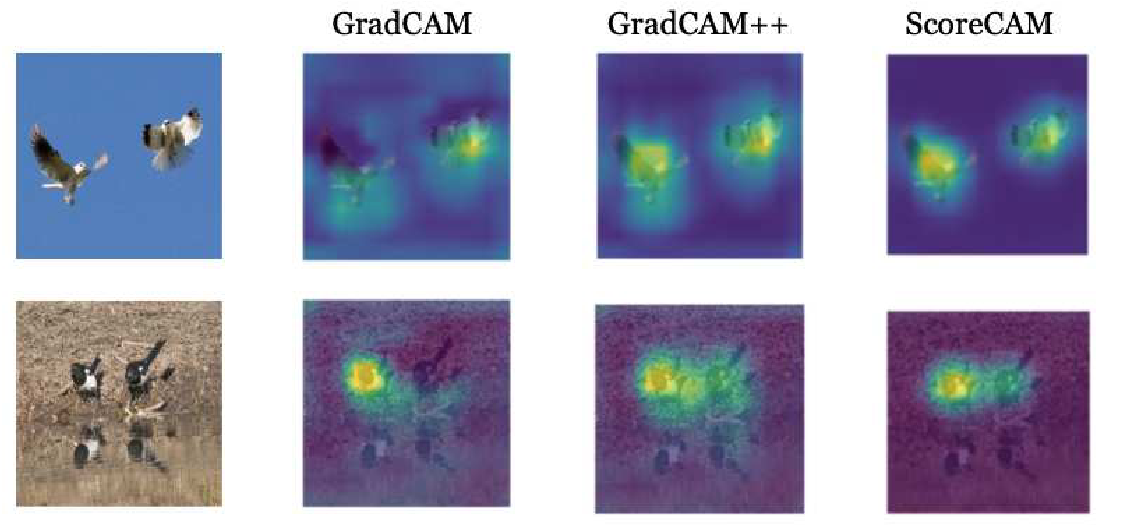
\includegraphics[width=0.5\linewidth]{Figures/scorecam_introduced_example.png}
    \caption{Images displaying the results of Score-CAM analysis.  This examples highlight the performance of Score-CAM when there are multiple objects from a given class present in the image.  Image taken from \citep{wang2020score}}
    \label{fig:scorecam_introduced}
\end{figure}








